\chapter{Conceptos básicos}

\label{BasicConcepts}

\section{Redes neuronales}
% TODO
Introducción a las redes neuronales, back-propagation, capas, input-outpus, etc


\section{Imágenes digitales}

Una imagen en el ámbito digital se entiende como una matriz de puntos.
Cada uno de estos puntos puede ser interpretado como un número real entre 0 y 1, que representa la localización de este punto en la escala de grises. En esta representación usaremos valores menores para los puntos más oscuros y valores mayores para puntos más claros.

Un ejemplo de esa representación es la matriz de la figura \ref{Seven_number}, que representa la imagen de la figura \ref{Seven_corner}.

\begin{figure}
    \centering
    \caption{\textit{Imagen resultante de la matriz}}
  \label{Seven_number}
  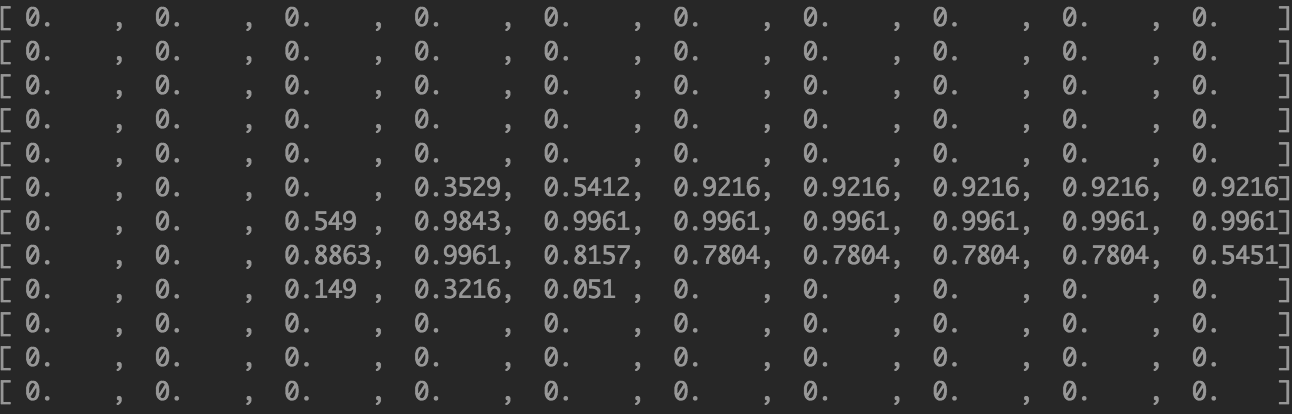
\includegraphics[width=\textwidth]{Seven_number}
\end{figure}

\begin{figure}
    \centering
    \caption{\textit{Imágen parcial en blanco y negro de un digíto escrito a mano}}
  \label{Seven_corner}
  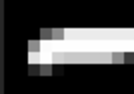
\includegraphics[width=.6\textwidth]{Seven_corner}
\end{figure}

En imágenes en color se suele usar el sistema \textit{RGB (Red, Green, Blue)} para representar diferentes colores en cada punto de la imagen. En vez de usar un solo valor por punto se usan tres valores, cada uno representando la intensidad del color rojo, verde y azul en ese punto. Superponiendo estos tres valores se consigue el color final. Por lo tanto, las imágenes \textit{RGB} constan de tres matrices, cada una con los valores reales entre 0 y 1 para cada color.

Para simplificar, algunos ejemplos de esta memoria van a usar una escala de grises, pero son aplicables a imágenes en color aplicando las operaciones a las tres diferentes capas al mismo tiempo.

\section{Filtros convolucionales}

Al trabajar con esta interpretación de lo que es una imagen, se pueden usar operaciones sobre la matriz de la imagen para transformarla de diferentes maneras.

Teniendo en cuenta cómo se representan, es claro que las imágenes digitales se pueden transformar mediante operaciones matriciales.

Consideremos la siguiente matriz 3$\times$3 (llamada matriz filtro de convolución):

\[
  F=
  \left[ {\begin{array}{ccc}
   -1 & -1 & -1 \\
   1 & 1 & 1 \\
   0 & 0 & 0 \\
  \end{array} } \right]
\]

Se puede usar $F$ como un filtro para una imagen de la siguiente manera: primero, superponemos la matriz en algún punto de la imagen. Esto modificará el pixel donde ha quedado colocado el valor central de la matriz F. Para ello multiplicamos cada uno de los valores superpuestos, sumamos los resultados y los sustituimos en el valor central. Esto se hace para cada píxel de la imagen original (superponer el filtro en ese píxel y sustituir el valor por la operación).

En los bordes de la matriz existen menos píxeles adyacentes a cada píxel: seis en los bordes y tres en las esquinas. Para que la operación se haga con la misma cantidad de elementos se presupone que todos los valores que no existen son 0.

En el caso de la matriz F, la fila superior son todos valores negativos, la intermedia son todos 1 y la inferior todos ceros. Si aplicamos entonces la operación descrita sobre una imagen, los píxeles más brillantes (aquellos con mayor valor) en la imagen resultante serán los que su fila superior es cero, eliminando los valores negativos y su fila intermedia es 1. 

Esto ocurrirá con más frecuencia en los bordes superiores de objetos claros con fondo oscuro.

Para mostar la utilidad de los filtros, los aplicaremos a la imagen de un dígito escrito a mano, sacado de la base de datos MNIST \parencite{lecun-mnisthandwrittendigit-2010}, que incluye 70000 imágenes de dígitos alfanuméricos escritos a mano.
\begin{center}
  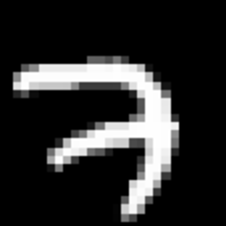
\includegraphics{seven}
\end{center}

Si aplicamos el filtro F a la imagen podemos observar cómo resalta en blanco los bordes superiores y en negro los inferioes. Filtros similares, rotando los valores del filtro F, son capaces de resaltar bordes laterales u oblicuos.

\begin{center}
  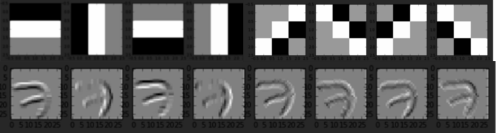
\includegraphics{filters}
\end{center}

Lo interesante de este método es que hemos conseguido resaltar características del objeto representado en la imagen simplemente con operaciones matricialessimplemente con operaciones matriciales.

Las matrices de convolución pueden ser de mayor tamaño, permitiendo capturar características más complejas. La matriz de 3$\times$3 es la menor matriz que permite definir en su totalidad el concepto de espacio, pudiendo extraer características espaciales en dos dimensiones.

A la hora de trabajar con imágenes en color es necesario usar un modelo de color. Uno de los más usados, RGB, se compone de tres capas, una dedicada a la intensidad roja, otra a la verde y la última a la azul, de ahí su nombre. Cada filtro se aplicaría a cada capa por separado, permitiendo de esta manera detectar diferentes características de la imagen que ocurran solo en uno de los colores.

Para analizar cómo afectan diferentes filtros a una imagen, existe una página \parencite{visualizer_convolution} donde se pueden probar ejemplos con filtros personalizados, haciendo el concepto mucho más sencillo de comprender.

\section{Redes neuronales convolucionales}
\label{sec:conv-net}

Hemos explorado la idea de que determinados filtros son capaces de extraer información localizada sobre características de la imagen. En el ejemplo del apartado anterior, dada una imagen podíamos saber si había bordes superiores y dónde se podían encontrar. Esto puede ser de gran utilidad en el campo de reconocimiento de imágenes, ya que podemos usar esa información localizada para categorizar o aplicar otro tipo de técnicas en esas áreas señaladas.

El problema está en cómo encontrar los mejores filtros para sacar las características más relevantes de una imagen.

Analizando como funcionan los filtros convolucionales vemos su parecido con las redes neuronales. Al igual que las redes neuronales, los filtros son matrices que estamos aplicando a los datos de entrada que producirán unos datos de salida relevantes con la función buscada. El entrenamiento de una red neuronal va modificando los pesos de las diferentes capas hasta que produce una salida relevante con los ejemplos del conjunto de entrenamiento.

Si entendemos los pesos como la matriz convolucional, podemos hacer que sea la misma red la que busque el mejor filtro para nuestro problema de clasificación. De hecho, ya que las redes neuronales son capaces de componer diferentes funciones en diferentes capas de la red para imitar funciones no lineales, podemos aplicar la misma idea a las redes con filtros: componer diferentes filtros para poder extraer características más complejas.

En esta idea se basan las redes convolucionales que trabajan con imágenes. Cada capa de la red va a aplicar varios filtros a la imagen y a devolver las imágenes tratadas por dicho filtro para pasarlo a la siguiente capa. Ya que lo que importa es la composición de filtros, cada capa deberá entrenar varios filtros al mismo tiempo, permitiendo así aumentar la combinatoria final.

\begin{center}
  \makebox[\textwidth]{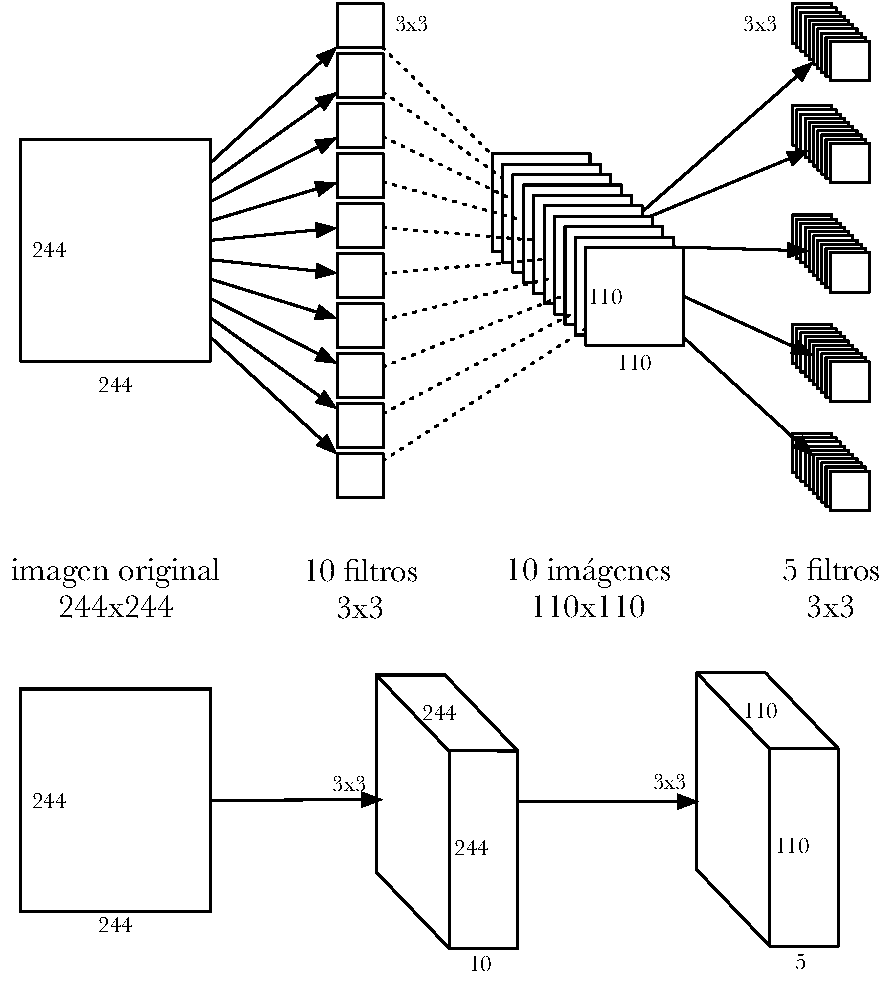
\includegraphics[width=\linewidth]{cnn}}
\end{center}

La manera de representar esto es entendiendo los pesos de cada capa como una matriz de tres dimensiones. Estas tres dimensiones se pueden entender como $d$ (profundidad) filtros de dimensión  $w \times h$ (anchura y altura). Cada capa tendrá su conjunto de filtros.

\subsection{Estructura de una capa convolucional}

El concepto de capa en una red convolucional incluye una agrupación de diferentes capas que efectúan diferentes operaciones. Como en las redes neuronales clásicas, la capa precisará de un tratamiento de las entradas con los pesos (en este caso los filtros convolucionales), y una función de activación aumentar la relevancia de las activaciones. 

\subsubsection{Capa convolucional - CONV \textit{(Convolutional layer)}}

Las capas convolucionales son las que hemos visto hasta ahora. Tendrán como pesos $n$ filtros convolucionales (todos del mismo tamaño), y producirán las $n$ salidas de aplicar la imagen de entrada a estos filtros. Una imagen de tamaño $32\times 32$ aplicada sobre una capa convolucional de 8 filtros producirá una salida de tamaño $32 \times 32 \times 8$, o lo que es lo mismo, 8 imágenes de $32 \times 32$

\subsubsection{Capa de activación - RELU \textit{(Rectifier Linear layer)}}
\label{sec:relu}

Al igual que en las redes clásicas es necesario tratar la salida de la aplicación de los pesos sobre las entradas con una función de activación. 

La manera estándar de modelar la salida de una neurona en las RNAs es a través de $f(x) = tanh(x)$ o $f(x) = (1 + e^{-x})^{-1}$ (función sigmoide). A la hora de entrenar la red con descenso del gradiente, estas funciones mucho más lentas que otra función que también evita la linealidad: $f(x) = max(0, x)$, llamada ReLU (\textit{Rectifier Linear}). Las redes neuronales convolucionales entrenan varias veces más rápido usando ReLU (ver figura \ref{relu-vs-tanh}) que las equivalentes usando la función $tanh$ \parencite{krizhevsky2012imagenet}

\begin{figure}
    \centering
    \caption{Evolución de un entrenamiento para una red convolucional de cuatro capas usando ReLUs (línea sólida) vs usando tanh (línea discontínua) \parencite{krizhevsky2012imagenet}}
  \label{relu-vs-tanh}
  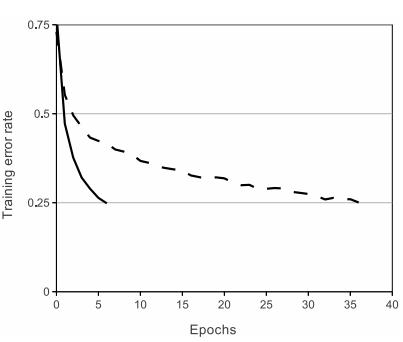
\includegraphics[width=.6\textwidth]{relu-vs-tanh}
\end{figure}

\subsubsection{Capa de muestreo - POOL \textit{(Pooling layer)}}

Al usar convoluciones en la imagen sobre el entorno de cada punto la información relevante de este queda difuminada y redundante. Gracias a esto se puede reducir el tamaño del problema mediante muestreo.
Las capas de muestreo (\textit{pooling layers}) resumen las salidas del entorno de cada grupo de neuronas. Un ejemplo de función de muestreo sería elegir el valor máximo de cada cuadrado de 4 píxeles (figura \ref{maxpool})

Si la salida de una capa CONV + RELU es $32 \times 32 \times 8$, al aplicar la capa de muestreo, la salida se convertirá en $16 \times 16 \times 8$. Al eliminar el 75\% de las activaciones se reducen la cantidad de parámetros y el tiempo de computación, y además ayuda a reducir el sobreajuste.

\begin{figure}
    \centering
    \caption{\textit{Max-pooling sobre una imagen de $4\times4$}}
  \label{maxpool}
  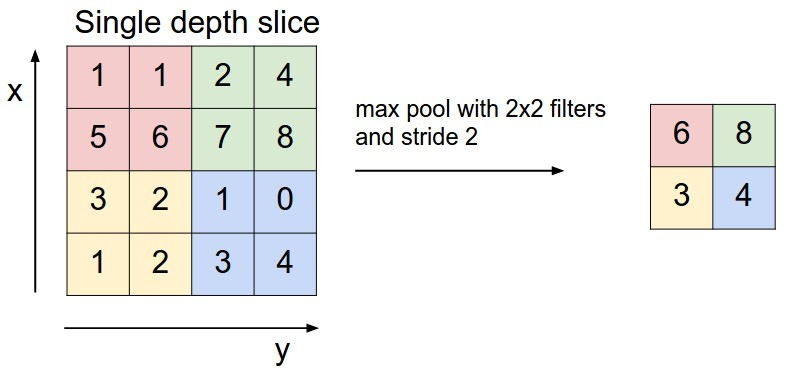
\includegraphics[width=.6\textwidth]{maxpool}
\end{figure}

\subsubsection{Capa densa - FC \textit{(Fully connected layer)}}

Esta capa es una capa clásica de red neuronal. Su función es calcular las probabilidades de clasificación dadas las imágenes tratadas. Cada neurona de esta capa estará conectada a cada una de las activaciones de la capa anterior, produciendo una salida por cada clase a clasificar.

Esta capa suele usarse al final de la arquitectura, cuando se han producido varios ciclos de capas convolucionales (CONV + RELU + POOL). Sin embargo, también es común ver arquitecturas con varias capas FC conectadas al final, ampliando la flexibilidad de clasificación de la red en base a características extraidas.

\subsection{Arquitectura}
\label{sec:conv-net-arch}

\begin{figure}
    \centering
    \caption{Ejemplo de arquitectura de una red convolucional para clasificación, \parencite{clarifai}}
\label{conv-arch}
  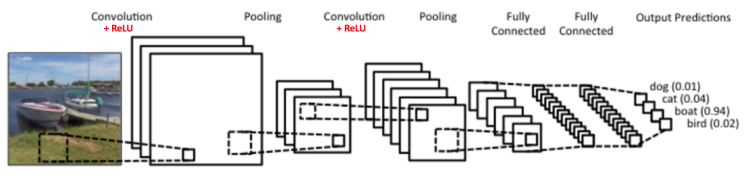
\includegraphics{conv-arch}
\end{figure}

Un esquema simplificado de un ejemplo de uso de las capas mencionadas se puede encontrar en la figura \ref{conv-arch}. La idea es, mediante capas CONV + RELU + POOL, transformar la imagen en una multitud de representaciones de conceptos cada vez más abstractos. Una vez se alcancen dichos conceptos, usar capas FC para modelar la salida de la red.

Como se verá en la solución presentada para este proyecto, en el capítulo \ref{cap:soluciones}, usar esta arquitectura permite apoyarse en determinadas estrategias para mejorar la eficacia del modelo predictivo.
